% !TeX encoding = UTF-8
% !TeX program = pdflatex
% !TeX spellcheck = it_IT

\documentclass[Lau,binding=0.6cm,noexaminfo=true]{sapthesis}

\usepackage{microtype}
\usepackage[italian]{babel}
\usepackage[utf8]{inputenx}

\usepackage{hyperref}
\hypersetup{pdftitle={Analisi delle problematiche di sicurezza del protocollo MQTT},pdfauthor={Edoardo Di Paolo}}

% Remove in a normal thesis
\usepackage{lipsum}
\usepackage{curve2e}
\usepackage{setspace}
\onehalfspacing

%code related
\usepackage{pythonhighlight}


\definecolor{gray}{gray}{0.4}
\newcommand{\bs}{\textbackslash}

% Commands for the titlepage
\title{Analisi delle problematiche di sicurezza del protocollo MQTT}
\author{Edoardo Di Paolo}
\IDnumber{1728334}
\course{Informatica}
\courseorganizer{Facoltà di Ingegneria dell'informazione, informatica e statistica}
\AcademicYear{2019/2020}
\copyyear{2020}
\advisor{Prof. Angelo Spognardi}
%\advisor{Dr. Nome Cognome}
%\coadvisor{Dr. Nome Cognome}
\authoremail{dipaolo.1728334@studenti.uniroma1.it}

%\examdate{ }
%\examiner{ }
%\examiner{Prof. Nome Cognome}
%\examiner{Dr. Nome Cognome}
%\versiondate{\today}




\begin{document}

\frontmatter

\maketitle

\dedication{Dediche.\\}

%\begin{acknowledgments}
%Ringraziamenti
%\end{acknowledgments}


%\begin{abstract}
%Introduzione
%\end{abstract}


\tableofcontents

% Do not use the starred version of the chapter command!



\mainmatter
\chapter{Introduzione}

\begin{large}
Negli ultimi decenni il numero di dispositivi collegati ad Internet è cresciuto esponenzialmente. Ormai, nel 2020, non si hanno più solamente computer o cellulari in rete ma anche elettrodomestici, macchine industriali e strumenti medici, tutti dispositivi che qualche anno fa erano offline. Tutto ciò fa riferimento all'IoT, l'\textit{Internet of Things}. \\
Parallelamente allo sviluppo di queste nuove tecnologie, sono stati studiati nuovi protocolli affinché i dispositivi potessero essere utilizzati in maniera efficiente. Ad esempio ci sono alcuni sensori i quali permettono di misurare temperatura ed umidità di una stanza e funzionano attraverso l'uso di una semplice pila; dunque è necessario andare a ridurre il costo energetico della connessione così da aumentare la durata di utilizzo del dispositivo. \\
Alcuni esempi di protocolli possono essere: MQTT, CoAP, AMQP e WebSocket. Ovviamente tutti i protocolli hanno la possibilità di essere integrati con TLS (\textit{Transport Layer Security}) così da poter garantire una maggiore sicurezza nello scambio dei dati; questo, però, potrebbe andare a gravare sui consumi del dispositivo poiché dovrebbero essere effettuati più calcoli affinché avvenga il trasporto dei dati. Inoltre, con l'aumento di questi nuovi dispositivi sono aumentate anche le possibili minacce relative all'IoT. Un esempio è il malware Mirai \cite{wiki:Mirai} che, nel 2016, ha infettato milioni di dispositivi rendendoli parte di una botnet la quale, successivamente, ha attaccato attraverso un DDoS il fornitore di servizi DNS Dyn così da rendere inaccessibili milioni di siti web. A causa, anche, di questa tipologia d'attacco, sempre più comune, i protocolli sviluppati devono presentarsi sicuri e robusti.\\

In questa relazione viene descritto lo studio effettuato su uno dei maggiori protocolli nell'IoT: MQTT. Nello specifico durante l'attività di tirocinio siamo andati alla ricerca di possibili anomalie e/o violazioni del protocollo da parte dei broker server i quali dovrebbero rispettare ogni standard definito per MQTT.

\end{large}


\chapter{MQTT}

\begin{large}

\section{Descrizione del protocollo}

MQTT, acronimo di \textit{Message Queuing Telemetry Transport}, è un protocollo di tipo \textit{publish-subscribe} il quale permette il trasporto di messaggi tra diversi dispositivi tramite TCP/IP. Il protocollo è molto utilizzato in ambito IoT per la sua semplicità e anche per la banda la cui richiesta è davvero bassa. \\

MQTT presenta un modello di architettura differente, ad esempio, dal tipico client/server del protocollo HTTP; infatti adotta il meccanisco \textit{publish-subscribe} (pub/sub) attraverso l'utilizzo di un \textit{broker}. Il funzionamento del modello pub/sub avviene attraverso la pubblicazione e la sottoscrizione da parte del client a diversi topic, che possono essere paragonati a dei canali di comunicazione. In MQTT il publisher e il subscriber non comunicano mai direttamente e non sono neppure consapevoli della presenza dell'uno e dell'altro: il collegamento è gestito dal broker il cui compito è quello di filtrare i messaggi che riceve e distribuirli ai vari subscribers. 
In questo capitolo sono analizzate le principali caratteristiche che il protocollo MQTT mette a disposizione.
%shodan stats (?)

\subsection{Topic}
Nel protocollo MQTT un topic non è altro che una stringa codificata in UTF-8 che il broker utilizza per filtrare i messaggi da inviare successivamente ad ogni client sottoscritto a quel topic. I topic sono case-sensitive, quindi bisogna prestare attenzione alle lettere maiuscole o minuscole, e la lunghezza minima dev'essere di un carattere. Inoltre, MQTT mette a disposizione del client dei \textit{wildcard}, i quali permettono di connettersi simultaneamente a più topic; uno è rappresentato dal simbolo +, mentre l'altro dal simbolo \#. Il primo è chiamato \textit{single-level} wildcard, mentre il secondo \textit{multi-level} wildcard. Ci sono dei topic, a cui non si può pubblicare alcun messaggio, riservati allo stato del sistema e sono quei topic che cominciano per \$SYS/. \\
Alcuni esempi di topic validi possono essere i seguenti: 
\begin{enumerate}
\item \textit{casa/luci/sala} - topic specifico per le luci della sala;
\item \textit{casa/+/sala} - include tutti i topic dei dispositivi che fanno riferimento alla sala (luci comprese);
\item \textit{casa/\#} - include tutti i topic che fanno riferimento alla casa.
\end{enumerate}


\subsection{Connessione al broker}
Come scritto nell'introduzione di questo capitolo, la connessione avviene solamente fra client e broker. Per client intendiamo un qualsiasi dispositivo il quale permette di gestire una connessione ad un broker, che si comporta come un server. 

\begin{figure}[h]
\centering

\includegraphics[width=0.7\textwidth]{images/connect-connack.png}
\caption{Flusso connessione al broker MQTT.}
\label{fig:connect-connack}
\end{figure}

Come si può vedere dalla Figura \ref{fig:connect-connack}, la connessione avviene tramite lo scambio di due pacchetti: \textit{connect}, inviato dal client al broker, e \textit{connack} inviato dal broker al client. Il pacchetto connect è così strutturato:
\begin{table}[h]
\caption{Struttura pacchetto connect.}
\label{tab:connect}
\begin{tabular}{lp{0.8\textwidth}}
\toprule
\textbf{Parametro} & \textbf{Descrizione} \\
\midrule
\textit{clientId} & rappresenta l'identificativo del client che chiede di connettersi \\
\textit{cleanSession} & valore booleano il quale specifica se la connessione è persistente o meno \\
\textit{username} & rappresenta l'username necessario affinché avvenga la connessione \\
\textit{password} & la password associata all'username \\
\textit{willRetain} & viene letto solo se \textit{willFlag} è true \\
\textit{willQos} & viene letto solo se \textit{willFlag} è true \\
\textit{willFlag} & permette di notificare un messaggio specificato dal client nel payload in caso di disconnessione anomala \\
\textit{keepAlive} & rappresenta in secondi l'intervallo massimo in cui broker e client possono non inviarsi messaggi \\
\bottomrule
\end{tabular}
\end{table}

Il pacchetto connack, invece, è così strutturato: \\
\begin{table}[h]
\caption{Struttura pacchetto connack.}
\label{tab:connack}
\begin{tabular}{lp{0.8\textwidth}}
\toprule
\textbf{Parametro} & \textbf{Descrizione} \\
\midrule
\textit{sessionPresent} & flag riferita al cleanSession del pacchetto connect \\
\textit{returnCode} & stato della connessione \\
\bottomrule
\end{tabular}
\end{table}

Per quanto riguarda il \textit{returnCode} descritto nella Tabella \ref{tab:connack}, questo è un valore che va da 0 a 5:
\begin{itemize}
\item 0: connessione accettata;
\item 1: connessione rifiutata, versione del protocollo non valida;
\item 2: connessione rifiutata, clientId non valido;
\item 3: connessione rifiutata, server non disponibile;
\item 4: connessione rifiutata, username o password errati;
\item 5: connessione rifiutata, non autorizzati.
\end{itemize}

\subsection{Sottoscrizione e pubblicazione}
Come scritto più volte, MQTT è un protocollo che adotta un meccanismo chiamato \textit{publisher/subscribe}; perciò due aziono fondamentali che un client può compiere sono quelle chiamate \textit{publish} e \textit{subscribe}.
\subsubsection{Subscribe}
L'azione subscribe permette al client di sottoscriversi a un determinato topic passato nel pacchetto.

\begin{figure}[h]
\centering
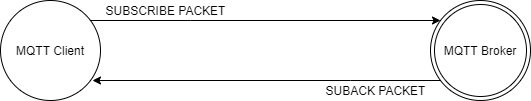
\includegraphics[width=0.7\textwidth]{images/subscribe-suback.png}
\caption{Flusso subscription ad un topic in MQTT.}
\label{fig:subscribe-suback}
\end{figure}

Come si nota dalla figura \ref{fig:subscribe-suback}, la sottoscrizione avviene semplicemente con lo scambio di due pacchetti: \textit{subscribe}, dal client al broker, e \textit{suback}, dal broker al client. Il primo pacchetto rappresenta la richiesta di sottoscrizione ad un determinato topic, il secondo invece conferma la sottoscrizione a quel topic. \\
La struttura del subscribe packet è la seguente:

\begin{table}[h]
\caption{Struttura pacchetto subscribe.}
\label{tab:subscribe}
\begin{tabular}{lp{0.8\textwidth}}
\toprule
\textbf{Parametro} & \textbf{Descrizione} \\
\midrule
\textit{packetId} & l'identificatore del pacchetto \\
\textit{payload} & una lista di QoS e topic a cui sottoscriversi \\
\bottomrule
\end{tabular}
\end{table}
Il pacchetto suback, invece, è così strutturato:
\begin{table}[h]
\caption{Struttura pacchetto subscribe.}
\label{tab:subscribe}
\begin{tabular}{lp{0.8\textwidth}}
\toprule
\textbf{Parametro} & \textbf{Descrizione} \\
\midrule
\textit{packetId} & l'identificatore del pacchetto a cui rispondere \\
\textit{returnCode} & lista di \textit{returnCode} che rappresentano lo stato della sottoscrizione \\
\bottomrule
\end{tabular}
\end{table}

Anche in questo caso il \textit{returnCode} può assumere diversi valori, riassunti in questa lista:
\begin{enumerate}
\item 0: successo, massimo QoS 0;
\item 1: successo, massimo QoS 1;
\item 2: successo, massimo QoS 2;
\item 128: sottoscrizione fallita.
\end{enumerate}

All'azione di sottoscrizione corrisponde anche un'azione di disiscrizione dal topic che avviene attraverso il pacchetto \textit{unsubscribe}. Quest'ultimo è così strutturato:
\begin{table}[h]
\caption{Struttura pacchetto unsubscribe.}
\label{tab:unsubscribe}
\begin{tabular}{lp{0.8\textwidth}}
\toprule
\textbf{Parametro} & \textbf{Descrizione} \\
\midrule
\textit{packetId} & l'identificatore del pacchetto a cui rispondere \\
\textit{topics} & lista di topic da cui disiscriversi \\
\bottomrule
\end{tabular}
\end{table}

\subsubsection{Publish}
La pubblicazione di un messaggio in MQTT è più complicata rispetto alla fase di sottoscrizione al topic. Prima di tutto, bisogna introdurre il concetto di QoS, \textit{Quality of Service}. Il QoS è paragonabile ad un contratto che viene stipulato tra client e broker; esistono tre diversi livelli: QoS 0, QoS 1, QoS 2.


Nel Quality of Service di livello 0 il payload del pacchetto viene pubblicato immediatamente. In questo caso non c'è garanzia sull'effettiva pubblicazione del messaggio.
\begin{figure}[h]
\centering
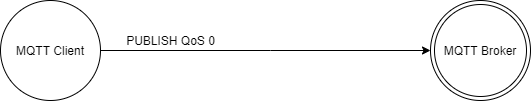
\includegraphics[width=0.7\textwidth]{images/publish-qos0.png}
\caption{Flusso publish con QoS 0.}
\label{fig:qos-0pub}
\end{figure}

Nel caso del Quality of Service di livello 1 viene garantita la pubblicazione ad almeno un destinatario.
\begin{figure}[h]
\centering
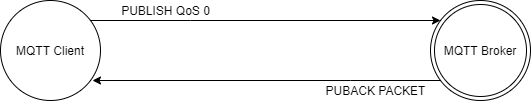
\includegraphics[width=0.7\textwidth]{images/publish-qos1.png}
\caption{Flusso publish con QoS 1.}
\label{fig:qos-1pub}
\end{figure}

Come si vede dalla Figura \ref{fig:qos-1pub}, il client riceve dal broker il pacchetto \textit{puback} solo dopo aver pubblicato il pacchetto publish. 
Il pacchetto puback è così strutturato:
\begin{table}[h]
\caption{Struttura pacchetto puback.}
\label{tab:puback}
\begin{tabular}{lp{0.8\textwidth}}
\toprule
\textbf{Parametro} & \textbf{Descrizione} \\
\midrule
\textit{packetId} & l'identificatore del pacchetto publish \\
\bottomrule
\end{tabular}
\end{table}

Questo meccanismo permette al client di inviare nuovamente il pacchetto publish nel caso in cui, dopo un certo intervallo di tempo, non abbia ancora ricevuto il puback dal broker; in questo caso, nel pacchetto publish, il campo \textit{dup} sarà impostato come true. Inoltre, il client mantiene in memoria il pacchetto publish finché non riceve il puback.

Infine abbiamo il QoS di livello 2 il quale dà maggiore affidabilità ma è più lento rispetto ai precedenti livelli.

\begin{figure}[h]
\centering
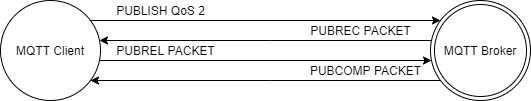
\includegraphics[width=0.7\textwidth]{images/publish-qos2.png}
\caption{Flusso publish con QoS 2.}
\label{fig:qos-2pub}
\end{figure}

Come si vede dalla Figura \ref{fig:qos-2pub} abbiamo più messaggi scambiati fra client e broker. Questo meccanismo assicura che il messaggio sia ricevuto solamente una volta dai destinatari; il livello 2, perciò, dà un maggiore livello di sicurezza al client.
Nel caso in cui il pacchetto vada perso, dopo un certo intervallo di tempo il client trasmetterà nuovamente il pacchetto e resterà in attesa della risposta da parte del broker. \\
La struttura dei pacchetti è la stessa che si può vedere nella Tabella \ref{tab:puback}. \\

Adesso che sono stati analizzati i differenti QoS, si può analizzare nel dettaglio il publish, il pacchetto più complicato del protocollo.
Il pacchetto ha i seguenti campi:
\begin{table}[h]
\caption{Struttura pacchetto publish.}
\label{tab:publish}
\begin{tabular}{lp{0.8\textwidth}}
\toprule
\textbf{Parametro} & \textbf{Descrizione} \\
\midrule
\textit{packetId} & l'identificatore del pacchetto \\
\textit{topic} & il topic a cui si vuole pubblicare il messaggio \\
\textit{qos} & il Quality of Service del pacchetto \\
\textit{retainFlag} & booleana per il \textit{retained} \\
\textit{payload} & il contenuto del messaggio \\
\textit{dup} & booleana che indica se il messaggio è un duplicato \\
\bottomrule
\end{tabular}
\end{table}

Dopo aver ricevuto il pacchetto il broker processa il messaggio in base al QoS; una volta processato invia il pacchetto a tutti i client sottoscritti al topic.

\begin{figure}[h]
\centering
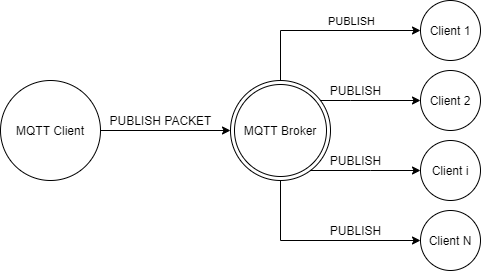
\includegraphics[width=0.7\textwidth]{images/publish-flow-example.png}
\caption{Esempio di pubblicazione di un pacchetto.}
\label{fig:publish-flow-example}
\end{figure}

\subsection{Altre caratteristiche}
\subsubsection{Retained message}
Un \textit{retained message} è semplicemente un pacchetto che ha impostato il valore true della \textit{retainFlag}. Di solito il broker una volta che riceve un messaggio da pubblicare su un topic, in cui nessun client è iscritto, lo scarta; questo avviene quando il retain è \textit{false}. Nel caso di un \textit{retained message} il broker salva in memoria il pacchetto che ha ricevuto per poi pubblicarlo una volta che un client si sottoscrive al topic.

\subsubsection{Last and will testament}
Questo meccanismo, indicato anche con \textit{LWT}, ci permette di gestire meglio le disconnessioni improvvise da parte di un client. Quando il dispositivo si connette al broker, nel pacchetto connect (Tabella \ref{tab:connect}), viene specificato il payload nel caso in cui avvenga una disconnessione imprevista; questo payload viene salvato dal broker il quale lo utilizzerà in caso di imprevisto.

\subsubsection{Clean session o persisted session}
Questa funzionalità viene specificata dal client nel momento della connessione; infatti nel pacchetto \textit{connect} (Tabelle \ref{tab:connect}) viene specificata una variabile \textit{cleanSession}. Nel caso di una persisted session il client riceverà dal broker tutti i messaggi pubblicati sui topic a cui si era sottoscritto che sono stati inviati mentre era offline.
\end{large}

\chapter{Implementazione ed esperimenti}
\begin{large}
Per ricercare possibili anomalie prodotte dalle librerie broker MQTT, c'è stata la necessità di implementare una libreria client la quale potesse permettere di gestire a basso livello i pacchetti e il loro flusso; infatti le librerie come \textit{paho} per python e \textit{mqtt.js} per nodejs non permettono di lavorare a basso livello.

\section{La libreria client}
La libreria client è stata scritta in python e utilizza la libreria \textit{twisted} \cite{wiki:Twisted}. 
Sono stati implementati tutti i pacchetti che MQTT mette a disposizione, inclusi tutti i livelli QoS. \\
Un esempio di pacchetto costruito è quello publish; i vari campi sono descritti nella Tabella \ref{tab:publish}, qui possiamo vedere il \textit{fixed header} del pacchetto.

\begin{table}[h]
\caption{Fixed header publish packet.}
\label{tab:publishbytes}
\centering
\begin{tabular}{|l|c|c|c|c|c|c|c|c|}
\hline
\textbf{bit}     & 7 & 6 & 5 & 4 & 3   & 2 & 1 & 0       \\
\hline
\textbf{byte 1}  & \multicolumn{4}{|c|}{Packet} & Dup & \multicolumn{2}{|c|}{QoS level} & Retain  \\
\hline
        & 0 & 0 & 1 & 1 & x   & \multicolumn{2}{|c|}{x} & x \\
\hline
\textbf{byte 2}~ & \multicolumn{8}{|c|}{Remaining Length}                                                       \\
\hline
\end{tabular}
\end{table}

Oltre a questo header, abbiamo il \textit{variable header} che contiene il nome del topic a cui si sta pubblicando e l'id del pacchetto. Infine c'è campo per il \textit{payload}, ovvero il contenuto del messaggio da pubblicare.
\newpage

Il codice python per la gestione di questo pacchetto è il seguente:

\begin{python}
def publish(self, topic, message, dup=False, qos=0, retain=False, messageId=None):
    header = bytearray()
    varHeader = bytearray()
    payload = bytearray()
    
    header.append(0x03 << 4 | dup << 3 | qos << 1 | retain)
    varHeader.extend(_encodeString(topic.encode("utf-8")))
    
    if qos > 0:
    	if messageId is None:
    		varHeader.extend(_encodeValue(random.randing(1, 65535)))
    	else:
    		varHeader.extend(_encodeValue(messageId))
    
    payload.extend(_encodeString(message.encode("utf-8")))
    header.extend(_encodeLength(len(varHeader) + len(payload)))
    
    self.transport.write(header)
    self.transport.write(varHeader)
    self.transport.write(payload)
\end{python}

Come si può vedere, il codice rispecchia la costruzione del pacchetto come definito nell'OASIS standard \cite{oasis:publish}. Innanzitutto vengono definiti i tre differenti campi: header (fixed header), varHeader (variable header) e infine payload. Si può notare come il messageId, che è l'identificatore del pacchetto, venga utilizzato solamente nel caso in cui il qos sia diverso da 0; in questo caso, infatti, dopo il publish dovrebbe esserci un ulteriore scambio di pacchetti tra broker e client che coinvolge l'id del pacchetto. \\
Infine viene aggiunto il payload, codificato in utf-8, e viene esteso il fixed header aggiungendo la lunghezza totale tra varHeader e payload. Il trasporto vero e proprio del pacchetto dal client al broker, invece, è gestito grazie alla libreria twisted attraverso il metodo \textit{write}. \\

In maniera del tutto analoga sono stati implementati tutti gli altri pacchetti. Attraverso questa libreria client si ha accesso alla costruzione del pacchetto, cosa non possibile nelle librerie come paho; ciò ha permesso di creare dei test particolari che hanno dato risultati differenti in base al broker utilizzato.

\end{large}


% bibliography
%\cleardoublepage
%\phantomsection
\bibliographystyle{sapthesis} % BibTeX style
\bibliography{bibliography} % BibTeX database without .bib extension

\end{document}
